\chapter{Virtualization: VRF, Part 3}\label{virtualization-vrf-part-3}

\section{Intro to VRF}\label{intro-to-vrf}

\begin{figure}
\centering
\pandocbounded{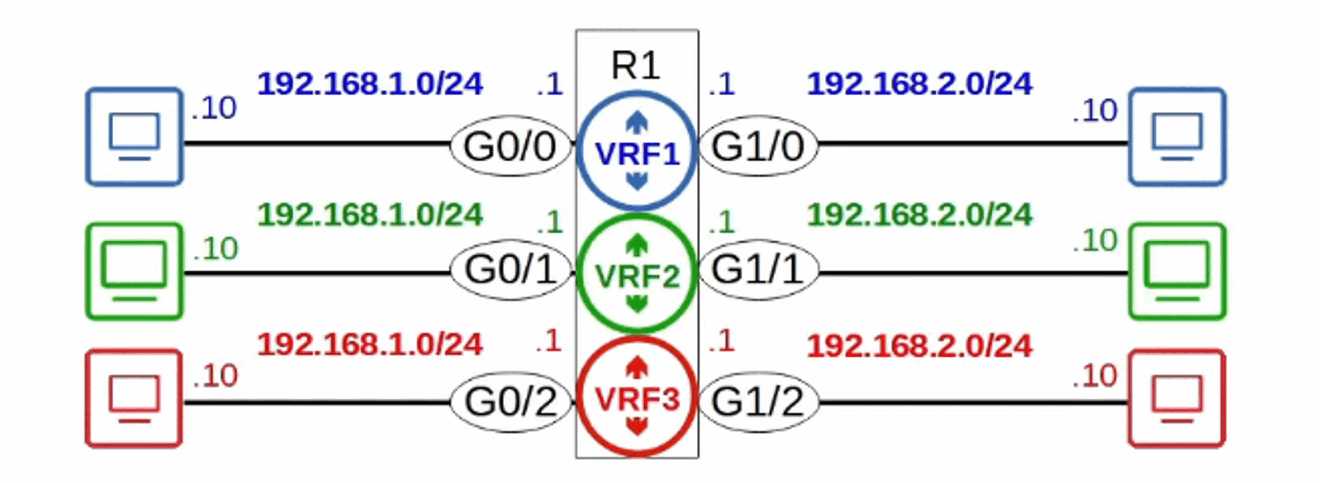
\includegraphics[keepaspectratio,alt={image}]{images/57-virtualization-vrf-part3/img-001.png}}
\end{figure}

\begin{itemize}
\tightlist
\item
  VIRTUAL ROUTING AND FORWARDING (VRF) is used to DIVIDE a SINGLE ROUTER
  into MULTIPLE VIRTUAL ROUTERS

  \begin{itemize}
  \tightlist
  \item
    Similar to how VLANs are used to divide a SINGLE SWITCH (LAN) into
    MULTIPLE VIRTUAL SWITCHES (VLANs)
  \end{itemize}
\item
  It does this by allowing a ROUTER to build MULTIPLE SEPARATE ROUTING
  TABLES

  \begin{itemize}
  \tightlist
  \item
    INTERFACES (LAYER 3 only) and ROUTERS are configured to be in a
    specific VRF (aka \emph{VRF INSTANCE})
  \item
    ROUTER INTERFACES, SVIs and ROUTED PORTS on MULTILAYER SWITCHES can
    be configured in a VRF
  \end{itemize}
\item
  TRAFFIC in one VRF cannot be forwarded out of an INTERFACE in another
  VRF

  \begin{itemize}
  \tightlist
  \item
    As an exception, VRF LEAKING can be configured to allow traffic to
    pass BETWEEN VRFs
  \end{itemize}
\item
  VRF is commonly used to facilitate MPLS (Multiple Protocol Label
  Switching)

  \begin{itemize}
  \tightlist
  \item
    The kind of VRF we are talking about is VRF-Lite (VRF without MPLS)
  \end{itemize}
\item
  VRF is commonly used by SERVICE PROVIDERS to allow ONE DEVICE to carry
  traffic from MULTIPLE CUSTOMERS

  \begin{itemize}
  \tightlist
  \item
    Each CUSTOMER'S TRAFFIC is isolated from the OUTSIDE
  \item
    CUSTOMER IP ADDRESSES can overlap without issue
  \end{itemize}
\end{itemize}

\section{VRF Configuration}\label{vrf-configuration}

\begin{figure}
\centering
\pandocbounded{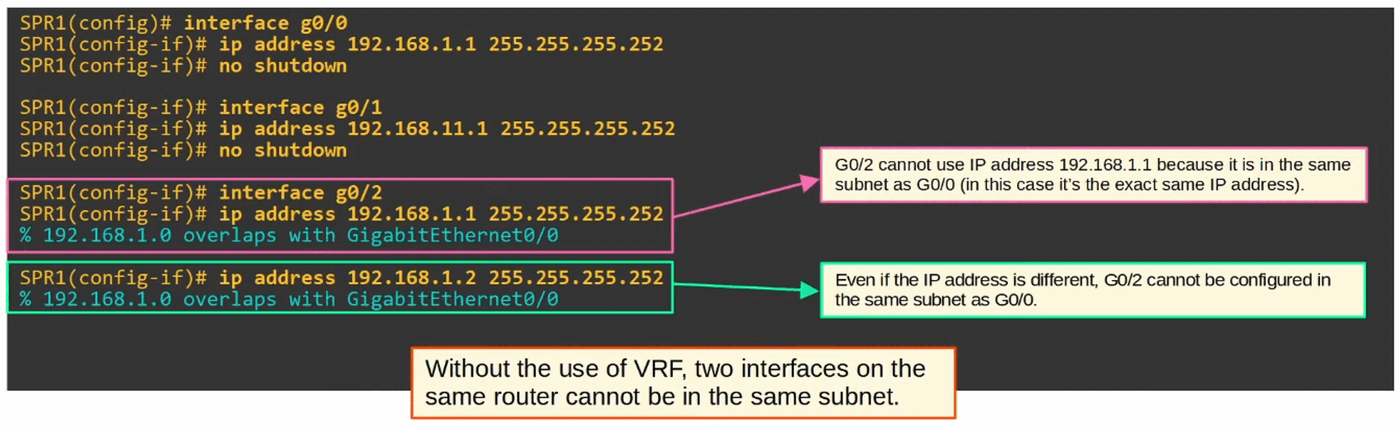
\includegraphics[keepaspectratio,alt={image}]{images/57-virtualization-vrf-part3/img-002.png}}
\end{figure}

Creation and Configuration of VRFs

\begin{figure}
\centering
\pandocbounded{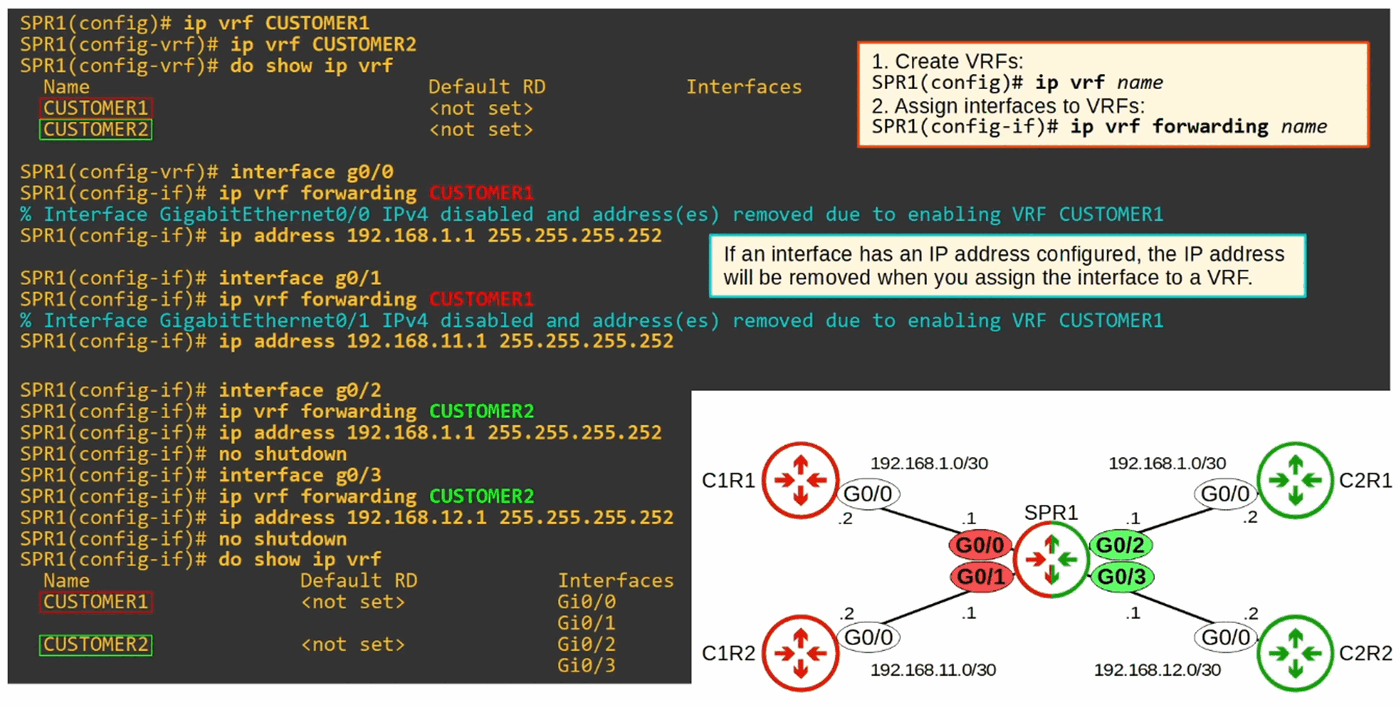
\includegraphics[keepaspectratio,alt={image}]{images/57-virtualization-vrf-part3/img-003.png}}
\end{figure}

How to \passthrough{\lstinline!show ip route!} for VRFs

\begin{figure}
\centering
\pandocbounded{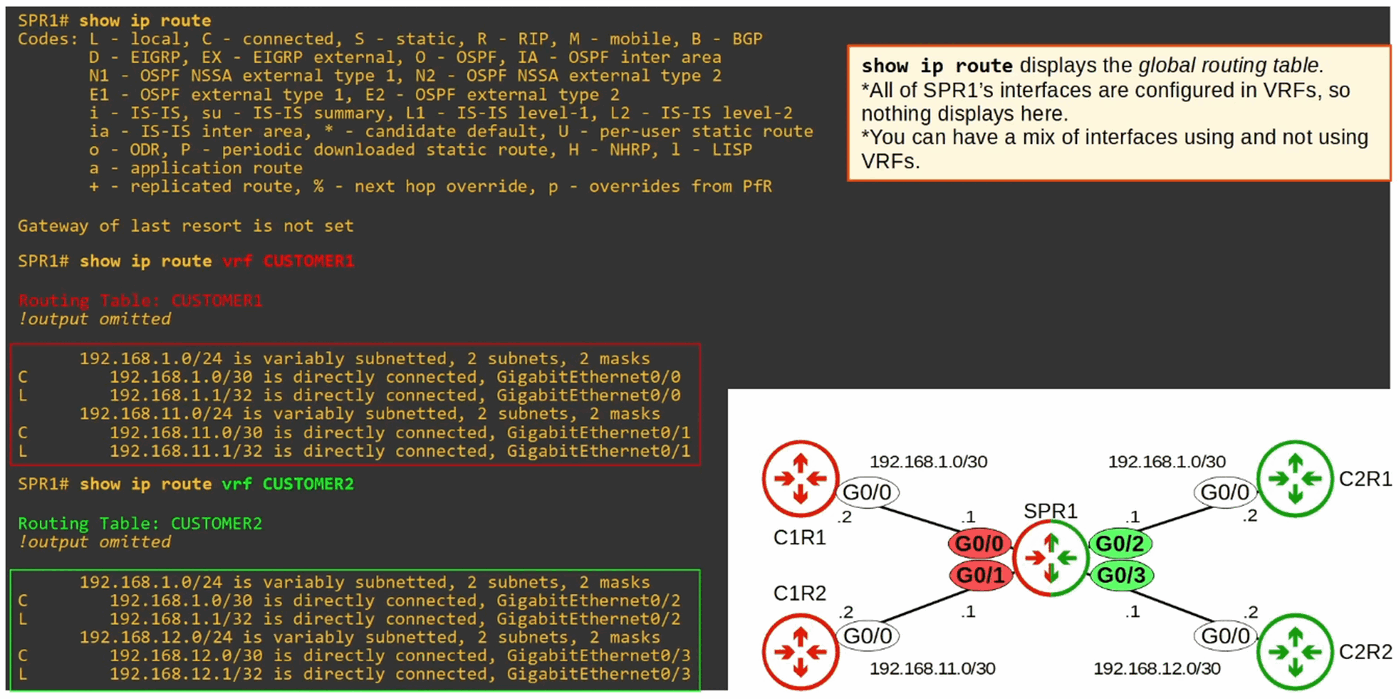
\includegraphics[keepaspectratio,alt={image}]{images/57-virtualization-vrf-part3/img-004.png}}
\end{figure}

\passthrough{\lstinline!ping!} other VRFs

\begin{figure}
\centering
\pandocbounded{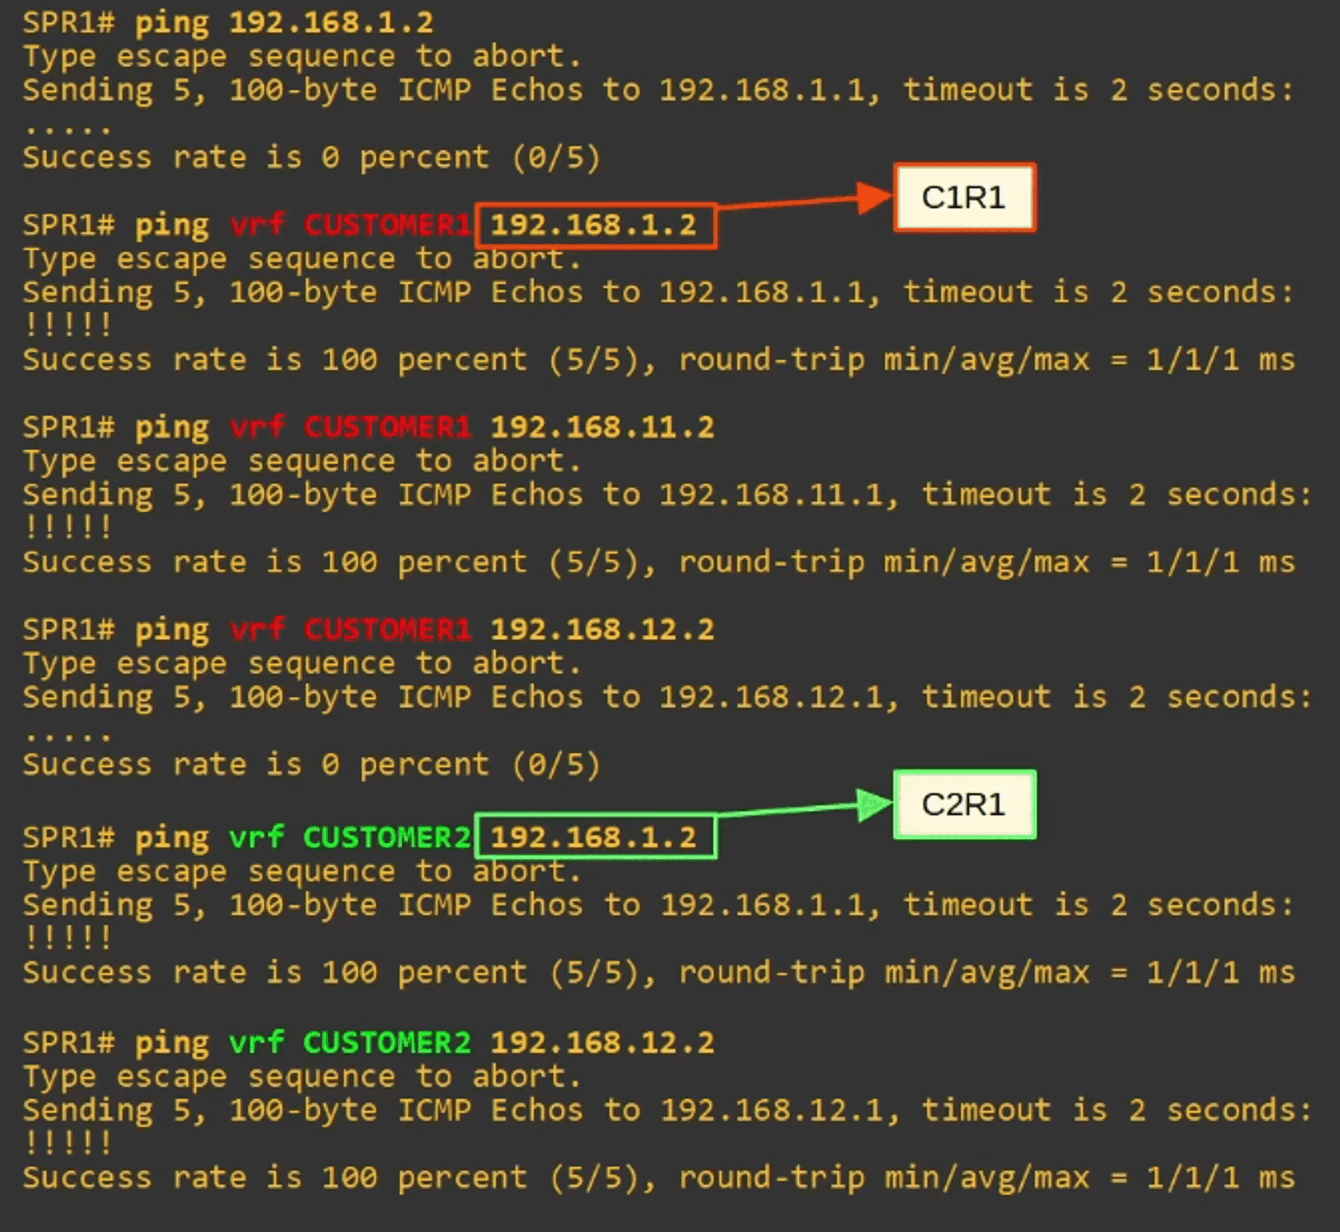
\includegraphics[keepaspectratio,alt={image}]{images/57-virtualization-vrf-part3/img-005.png}}
\end{figure}
